\begin{abstract}
We ask whether public scientific figures and captions improve a 4B vision--language model on AstroCLIMB. Supervised adaptation on graph-derived public pairs improves caption--image development macro-F1 in all three matched gold-training runs, with a mean gain of 0.0674. These runs share one public checkpoint. The submitted system combines separate modality classifiers and obtains a Kaggle public score of 0.75149. Increasing public adaptation from 2,000 to 4,000 updates improves paper-relation classification, but 8,000 updates bring no further gain. Neither answer generation nor the tested reinforcement-learning variants improve the selected classifier. Repeated development selection limits these findings to the evaluated setting.
\end{abstract}

\section{Introduction}

AstroCLIMB \citep{astroclimb} asks whether two scientific objects come from the same figure, the same paper, citation-related papers, or unrelated papers. Inputs comprise a caption--image pair (CXI), two images (IXI), or two captions (CXC); a citation in either direction defines related papers. Models must infer paper relations as well as figure--caption matches.

We investigate public figure--caption supervision before gold training. Starting from Qwen3.5-4B \citep{qwen35}, we train on graph-derived CXI pairs and then fit separate modality classifiers using low-rank adaptation (LoRA; \citealp{lora}). We compare public initialization with gold-only training under the same gold schedule, examine the effect of adaptation duration, and test alternatives to classification. The submitted system reaches four-class macro-F1 of \textbf{0.7562033665} on development and \textbf{0.75149} on the Kaggle public leaderboard. We make no rank claim.

\paragraph{Related work.}
Figure--caption correspondence \citep{lookreadenrich}, scientific image--text alignment in MedICaT \citep{subramanian-etal-2020-medicat}, figure captioning in SciCap \citep{hsu-etal-2021-scicap-generating}, and multimodal pretraining in SciOL \citep{sciol} use figures and text. SPECTER uses citations to learn document representations \citep{cohan-etal-2020-specter}. TRACS instead concerns telescope references and categorization \citep{grezes-etal-2025-overview}, so its scores are not comparable.

\section{Data and Evaluation}

\paragraph{Gold partitions.}
We reserve fold~1 of an inherited paper-component assignment for development and folds~2--4 for training; we do not independently reconstruct the split. After public-data duplicate checks, we retain 5,549 training pairs and 1,986 development pairs (Table~\ref{tab:data}). A separate 2,001-pair fold was seen in earlier experiments. We exclude it from further tuning and evaluation; it is not an untouched test.

\begin{table}[t]
\centering
\small
\begin{tabular}{lrr}
\hline
Input type & Training & Development \\
\hline
Caption--image & 2,230 & 794 \\
Image--image & 1,670 & 590 \\
Caption--caption & 1,649 & 602 \\
\hline
Total & 5,549 & 1,986 \\
\hline
\end{tabular}
\caption{Gold partitions after exposure filtering.}
\label{tab:data}
\end{table}

\paragraph{Public supervision.}
We index all 114 shards of \texttt{adsabs/AstroCLIMB}, covering 94,233 figures. Figure identity, paper identity, and observed citation edges define 80,000 balanced CXI training pairs and 2,000 public validation pairs. Unrelated examples mix random-paper, same-journal, and two-hop pairs without a direct edge. We do not manually verify these labels, and missing citation edges can produce noisy negatives.

Before generating pairs, we separate public validation components and remove whole gold training components that cross protected boundaries. Exclusion checks include label-free test content, using candidate paper identities, normalized captions, image-byte and decoded-pixel hashes, and 256-bit perceptual hashes within Hamming distance eight. Matches propagate through duplicate components and candidate-paper mappings. No matches remain under these checks, although missing metadata and unmatched objects limit identity recovery. Identifiers and hashes serve auditing only.

The classifier recipe uses no competition test labels. Earlier exploration nevertheless exposed released scoring information and a structural shortcut. We exclude the affected submissions and representations from this model lineage, but the benchmark was not wholly unseen at project level.

\paragraph{Selection and reporting.}
We select models on development data and use declared TRAIN-only monitors for feasibility trials. Development scores thus reflect repeated selection rather than unbiased estimation or nested cross-validation. Whole-task macro-F1 is computed from the pooled four-class confusion matrix. IXI and CXC contain no same-figure cases, so we also report their active-three-class macro-F1; the four-class logger assigns zero to the absent class. Public validation does not determine when adaptation stops.

\section{System}

\paragraph{Task-specific classifiers.}
We train one classifier per modality with Transformers \citep{wolf-etal-2020-transformers} and PEFT \citep{peft}. Each uses a frozen BF16 Qwen3.5-4B base, rank-16 LoRA (alpha 32, effective scaling 2), and a four-class head on the final non-padding representation. The adapters cover language MLP projections in all 32 layers and query, key, value, and output projections in the eight full-attention layers: about 21.2M parameters. The vision tower and linear-attention projections remain frozen. We use cross-entropy loss and zero adapter dropout.

CXI prompts contain an image and caption; IXI prompts contain Figure~A and Figure~B; CXC prompts contain two separated captions. We retain caption case and at most 2,400 characters per caption. Images are RGB-decoded from verified original bytes and limited to 262,144 pixels each. Prompts contain no paper identifiers or retrieved labels. For IXI and CXC, we mask the same-figure logit during training and prediction.

\paragraph{Public adaptation and gold specialization.}
Public adaptation precedes gold training only for CXI. We train on the balanced public corpus with batch size four, two accumulation steps, adapter/head learning rates of $10^{-4}$ and $3\!\times\!10^{-4}$, and a 10,000-update warmup/cosine schedule. The submitted model starts gold training from public update 4,000, after 32,000 pair presentations. The schedule itself remains 10,000 updates.

For gold training, CXI inherits the public adapter and head but uses a fresh optimizer. IXI and CXC start from the pristine base. Each uses batch size one, accumulation eight, three epochs, seed~7, and adapter/head learning rates of $3\!\times\!10^{-5}$ and $10^{-4}$. The resulting horizons are 837, 627, and 621 updates for CXI, IXI, and CXC. We select the highest development macro-F1 at epoch boundaries, breaking ties toward the earlier checkpoint. The submitted checkpoints are CXI837, IXI627, and CXC414.

\paragraph{Prediction and reproducibility.}
For IXI, we take the arithmetic mean of class probabilities for the original and reversed image order, as specified before evaluation. This improves development F1; the analogous caption-order average does not help CXC. We route each pair to its modality classifier and take the canonical-class argmax, without imposing test class counts. Submission uses the development-selected models directly, without an all-label final refit.

We preserve hashes of source, corpus, checkpoints, processors, and probability artifacts, and require fresh replay before accepting exports. Inference uses batch size one to match training. For the public2k-to-gold837 model, batch two changed 11 of 794 CXI predictions, with a maximum probability difference of 0.380. Source, configurations, and splits are prepared, but usable public checkpoints and independent end-to-end GPU reproduction remain incomplete.

\section{Results and Analysis}

\paragraph{Matched gold-only controls.}
We compare public initialization with gold-only training under identical gold schedules. Both arms run in the same RTX 3090 runtime with gold seeds 7, 19, and 37; only initialization differs. All six runs complete 837 updates. Fresh batch-one exports reproduce selected and final scores, with zero replay-logit discrepancy.

Public adaptation improves all three pairs (Table~\ref{tab:matched}). The mean gain is $0.06738$ for selected checkpoints and $0.06772$ at the final epoch. Both arms select update 558 for seed 19 and 837 otherwise. All runs share one public checkpoint, so this comparison tests variation in gold adaptation, not public pretraining. The public arm also uses additional compute. These fresh controls are not new Kaggle results.

\begin{table}[t]
\centering
\small
\begin{tabular}{rrrr}
\hline
Gold seed & Gold only & Public4k & Difference \\
\hline
7 & 0.68906 & 0.75619 & +0.06713 \\
19 & 0.67698 & 0.74811 & +0.07113 \\
37 & 0.68181 & 0.74569 & +0.06389 \\
\hline
\end{tabular}
\caption{Matched CXI controls on 794 DEV pairs, with epoch-boundary selection and one fixed public parent. Fresh runs, distinct from the submitted model.}
\label{tab:matched}
\end{table}

\paragraph{Public adaptation duration.}
The historical duration comparison also fixes the gold schedule. Increasing public adaptation from 2,000 to 4,000 updates raises CXI development macro-F1 from 0.70851 to 0.74839 (Figure~\ref{fig:results}a). Gains concentrate in paper relations: class F1 changes by $-0.005$ for same figure, $+0.052$ for same paper, $+0.072$ for related, and $+0.041$ for unrelated. On the same 794 pairs, this yields 81 corrections and 49 regressions.

More public training does not continue this improvement. At 8,000 updates, CXI scores 0.74285. Relative to 4,000, same-paper F1 falls by 0.049 while related and unrelated F1 rise by 0.018 and 0.011, with 45 corrections and 47 regressions. This class tradeoff does not establish a capacity ceiling.

\begin{figure*}[t]
\centering
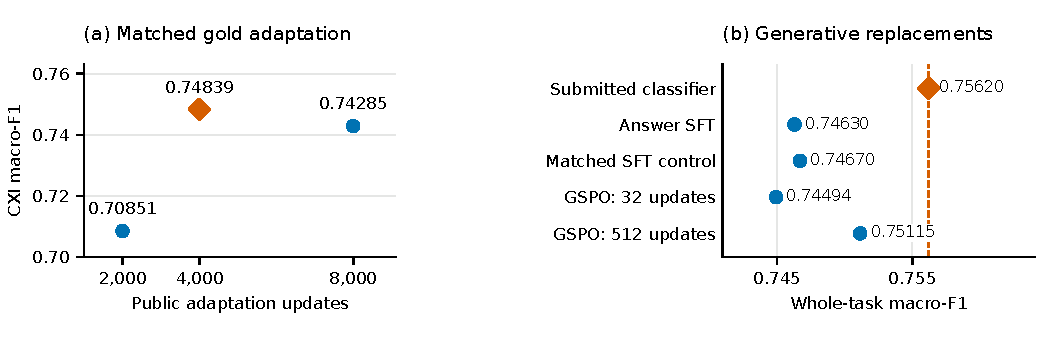
\includegraphics[width=\textwidth]{figures/results.pdf}
\caption{Development results, with zoomed score axes. (a) Public CXI adaptation followed by the same gold schedule; selected gold updates are 837, 837, and 279 respectively (794 pairs). (b) Generative CXI replacements with IXI/CXC fixed, scored on all 1,986 pairs. Orange diamonds mark the submitted choices. Points are single-seed selected results, not independent test estimates. GSPO runs differ in both context pool and update count.}
\label{fig:results}
\end{figure*}

\paragraph{Modality specialization.}
Separate gold training also improves IXI and CXC over their feature baselines. IXI reaches active-class F1 of 0.65536, against 0.54052 for frozen SigLIP~2 \citep{siglip2}/OCR features, and 0.67791 after image-order averaging. CXC reaches 0.72756, against 0.67277 for frozen Qwen3-Embedding-8B \citep{qwen3embedding} and BGE-base-en-v1.5 \citep{bgemodel,bgecpack} caption features. Caption-order averaging gives 0.72721, so we retain the original order. Together with the selected CXI branch, these classifiers score 0.75620 on pooled development data. Substituting the 8k CXI branch gives 0.75557, so we retain 4k.

\paragraph{Relation-level errors.}
Related-paper classification remains the weakest class in every modality. Pooled F1 is 0.92732 for same figure, 0.70809 for same paper, 0.58582 for related, and 0.80359 for unrelated. Confusions between same-paper and related-paper pairs account for 281 of 549 errors (51.2\%). This identifies a difficult decision boundary, but does not distinguish missing visual evidence from noisy graph supervision.

\paragraph{OCR and auxiliary transfer.}
OCR provides limited gains in the tested settings. Correctly aligned PP-OCRv6 \citep{ppocr6} features alone score 0.44142 on CXI. OCR-conditioned VLM adaptation falls slightly below the pristine gold-only VLM, although a fixed 50/50 combination improves an earlier whole-system baseline from 0.68987 to 0.69513. Public-to-gold transfer also fails to improve a separate frozen-feature IXI classifier, including in a matched-duration follow-up.

\paragraph{Generative training and reinforcement learning.}
We also test generation of relation labels. Using TRL \citep{trl}, we apply Group Sequence Policy Optimization (GSPO; \citealp{gspo}) to canonical answer generation. The classifier-adapted model initially produces only 13 strictly valid answers among 64 completions. We first train it to emit answer tags using 1,024 gold TRAIN pairs and 128 supervised updates.

GSPO uses batch size 16, four completions per context, two uses of each rollout, learning rate $10^{-6}$, group-normalized rewards, and zero reference-KL weight. Reward is one only for a correct canonical answer terminated by EOS; asymmetric clipping bounds are 0.0003 and 0.0004. Prediction uses the language-model output rather than the classifier head.

Both the 32- and 512-update runs complete verified parameter updates, but neither beats the classifier under the frozen full-development decision rule (Figure~\ref{fig:results}b). The 512-update model scores 0.75115, above answer-SFT (0.74630) and below the classifier (0.75620). Of its 26 corrections, 25 are related-paper cases; all 19 regressions fall outside that class. A matched 512-update SFT control is missing, so the gain over answer-SFT cannot be attributed specifically to reinforcement learning.

We then test whether more informative training examples help. Motivated by unanimous group rewards and dynamic sampling \citep{dapo}, a TRAIN-only trial compares 16 contexts with mixed outcomes among eight samples against 16 class-matched random contexts. Each receives 32 vLLM-assisted GSPO updates. Mixed selection increases informative groups from 14 to 24 of 32, but the frozen 256-context TRAIN monitor barely changes: 1,874 versus 1,875 correct answers out of 2,048. Neither meets the prospective two-percentage-point screen. More informative rollouts do not improve this monitor.

An isolated vLLM \citep{vllm} worker generates about 26.9 examples/s, versus 2.1--2.2 natively, on a fixed 64-example benchmark. Startup costs prevent an end-to-end speedup claim. Predictions also depend on the backend. We retain native inference as canonical and match batch shape and BF16 autocast across generation, scoring, and fresh-reload checks.

\paragraph{Sources of exploratory ideas.}
Visual-RFT and VLM-R1 \citep{visualrft,vlmr1} motivated verifiable visual rewards. Dr.~GRPO \citep{drgrpo} informed normalization discussions, but our trials retain GSPO. STaR \citep{star} suggested verified explanation bootstrapping, which we did not implement. Following the inspection idea in DeepEyes \citep{deepeyes}, we first tested fixed extra views. Three-vote accuracy on 64 TRAIN cases fell from 60/64 with repeated full views to 59/64 with one full view and two crops; we did not pursue learned inspection. Work on RL coverage and reasoning \citep{rlvrcoverage,rlvrreasoning} informed our distinction between sampled-answer and single-answer performance, without a general reasoning claim.

\section{Limitations and Conclusion}

Public adaptation improves CXI across three matched gold-training seeds. Longer adaptation trades class performance, and tested generative and reinforcement-learning alternatives do not surpass the classifier. The matched result is conditional on one public checkpoint; other neural comparisons use one seed.

Repeated development selection and previously exposed folds limit generalization claims. Incomplete citation graphs, imperfect identity recovery, and unknown base-model exposure further restrict interpretation. TRAIN monitors were exposed to ancestor models and serve as engineering screens, not independent test estimates.

Independent evaluation, public-pretraining seed replication, and better relation labels remain future work. Account-wide billing does not isolate experiment costs.
